\section{Introducción}
\begin{frame}
    \frametitle{Introducción}
    \begin{minipage}[c]{0.45\textwidth}
        
\includegraphics[width=\textwidth]{images/logo_gpul.png}
    \end{minipage}
    \hfill
    \begin{minipage}[c]{0.45\textwidth}
        
\includegraphics[width=0.6\textwidth]{images/logo_dafic.png}
    \end{minipage}
\end{frame}

\begin{frame}
    \frametitle{Un poco de historia (muy poco, lo prometo)}
    \begin{minipage}[c]{0.45\textwidth}
        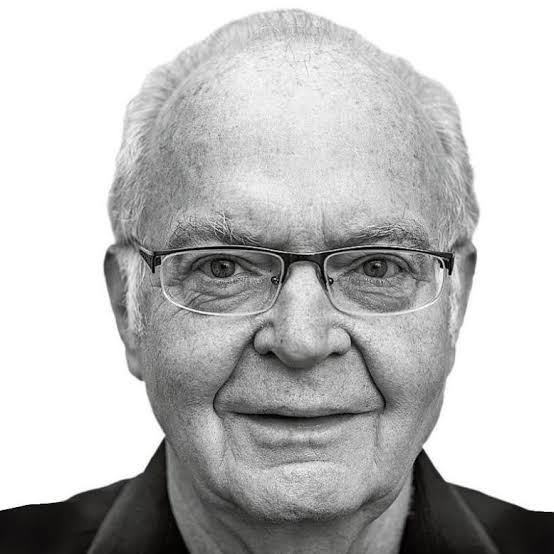
\includegraphics[width=\textwidth]{images/knuth.jpeg}
    \end{minipage}
    \hfill
    \begin{minipage}[c]{0.45\textwidth}
        \begin{itemize}
            \item{Donald Knuth, creador de \TeX en 1978}
            \item{A petición de la \emph{American Mathematical Society}}
            \item{¡Sigue siendo insustituible hoy en día!}
        \end{itemize}
    \end{minipage}
\end{frame}

\begin{frame}
\frametitle{¿\TeX = \LaTeX?}
\begin{itemize}
    \item{\textbf{Distribuciones:} \emph{MikTeX, TeX Live\dots}}
    \item{\textbf{Front ends (editores):} \emph{Overleaf}, \textbf{vim}\dots}
    \item{\textbf{Motores:} \emph{TeX}, \emph{pdfTeX}, \emph{LuaTeX}\dots}
    \item{\textbf{Formatos:} \emph{LaTeX}, \emph{TeX plano}\dots}
    \item{\textbf{Paquetes:} \texttt{transparent}, \texttt{geometry}\dots}
\end{itemize}
\end{frame}
